% !TEX program = xelatex
% Data Science — full course slide deck (16 sessions), Metropolis theme.
% Compile with:  latexmk -xelatex data-science-course.tex
\documentclass[10pt,aspectratio=169]{beamer}

\usetheme{metropolis}
\metroset{sectionpage=progressbar, numbering=fraction, progressbar=frametitle}

\usepackage{booktabs}
\usepackage{array}
\usepackage{tikz}
\usetikzlibrary{arrows.meta, positioning, shapes.geometric, fit, backgrounds}
\usepackage{tabularx}
\usepackage{amsmath}
\usepackage{amssymb}
\usepackage{adjustbox}

\setbeamertemplate{frame footer}{Data Science — a 16-session course}

% A light custom palette layered on top of Metropolis's defaults.
\definecolor{dsblue}{RGB}{27,94,150}
\definecolor{dsorange}{RGB}{214,109,25}
\definecolor{dsgreen}{RGB}{45,128,79}
\definecolor{dsred}{RGB}{175,45,45}
\definecolor{dsgray}{RGB}{90,98,107}
\setbeamercolor{palette primary}{bg=dsblue,fg=white}
\setbeamercolor{frametitle}{bg=dsblue,fg=white}
\setbeamercolor{progress bar}{fg=dsorange,bg=dsgray!30}

% Reusable "definition" and "warning" style blocks without extra packages.
\newcommand{\keyidea}[1]{%
  \begin{block}{}
  \centering\Large\bfseries\color{dsblue} #1
  \end{block}%
}
\newcommand{\trapbox}[2]{%
  \begin{alertblock}{\textbf{#1}}
  #2
  \end{alertblock}%
}
\newcommand{\analogybox}[2]{%
  \begin{exampleblock}{\textbf{Analogy --- #1}}
  #2
  \end{exampleblock}%
}

\title{Data Science}
\subtitle{From a raw file to a deployed model at scale}
\author{A 16-Session Course}
\date{}

\begin{document}

\maketitle

\begin{frame}{What this course covers}
\setlength{\itemsep}{0pt}
\begin{columns}[T]
\begin{column}{0.5\textwidth}
\textbf{Part A --- Getting hold of data}
\begin{itemize}\footnotesize
  \item S1 Introduction to Data Science
  \item S2 Data Collection \& Pre-Processing
\end{itemize}
\textbf{Part B --- Making data fit to use}
\begin{itemize}\footnotesize
  \item S3 Data Cleaning
  \item S4 Data Integration
  \item S5 Data Transformation
  \item S6 Data Reduction \& Discretization
\end{itemize}
\textbf{Part C --- Understanding data}
\begin{itemize}\footnotesize
  \item S7 Descriptive Statistics
  \item S8 EDA \& Visualization
\end{itemize}
\end{column}
\begin{column}{0.5\textwidth}
\textbf{Part D --- Learning from data}
\begin{itemize}\footnotesize
  \item S9 Supervised Learning
  \item S10 Unsupervised Learning \& Clustering
  \item S11 Model Evaluation
  \item S12 Model Saving \& Deployment
\end{itemize}
\textbf{Part E --- Data at scale}
\begin{itemize}\footnotesize
  \item S13 Big Data Fundamentals
  \item S14 Distributed Data Processing
  \item S15 NoSQL \& Visualization at Scale
  \item S16 Capstone Project
\end{itemize}
\end{column}
\end{columns}
\end{frame}

\begin{frame}{How the parts build on each other}
\begin{center}
\begin{adjustbox}{max width=0.94\linewidth, max height=4.6cm}
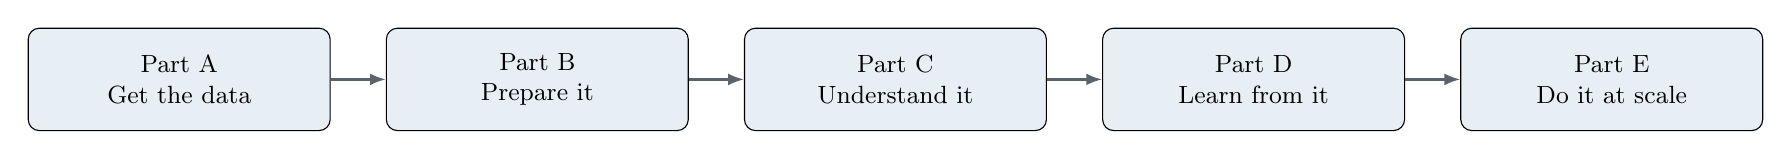
\begin{tikzpicture}[
  box/.style={draw, rounded corners, fill=dsblue!10, text width=3.6cm, align=center, minimum height=1.3cm, font=\small},
  arr/.style={-{Latex[length=2mm]}, thick, dsgray}
]
\node[box] (a) {Part A\\Get the data};
\node[box, right=0.7cm of a] (b) {Part B\\Prepare it};
\node[box, right=0.7cm of b] (c) {Part C\\Understand it};
\node[box, right=0.7cm of c] (d) {Part D\\Learn from it};
\node[box, right=0.7cm of d] (e) {Part E\\Do it at scale};
\draw[arr] (a) -- (b);
\draw[arr] (b) -- (c);
\draw[arr] (c) -- (d);
\draw[arr] (d) -- (e);
\end{tikzpicture}
\end{adjustbox}
\end{center}
\vspace{0.5cm}
\keyidea{You cannot model data you have not prepared, and you cannot prepare data you have not understood. Everything in this course follows that order.}
\end{frame}

% ============================================================
\part{Part A --- Getting Hold of Data}
\frame{\partpage}

\section{Session 1 --- Introduction to Data Science}

\begin{frame}{What is data science?}
\keyidea{Data science turns recorded facts into decisions.}
\vspace{0.3cm}
Three ingredients have to come together:
\begin{table}
\small
\begin{tabularx}{\linewidth}{@{}lXX@{}}
\toprule
\textbf{Ingredient} & \textbf{What it gives you} & \textbf{Without it} \\
\midrule
Programming & handle more rows than a person could ever read & stuck with what fits on one screen \\
Mathematics & tell a real pattern from a coincidence & find patterns in noise \\
Domain knowledge & know what the numbers \emph{mean} & correct answer to the wrong question \\
\bottomrule
\end{tabularx}
\end{table}
\end{frame}

\begin{frame}{The seven-stage lifecycle}
\begin{center}
\begin{adjustbox}{max width=0.94\linewidth, max height=4.6cm}
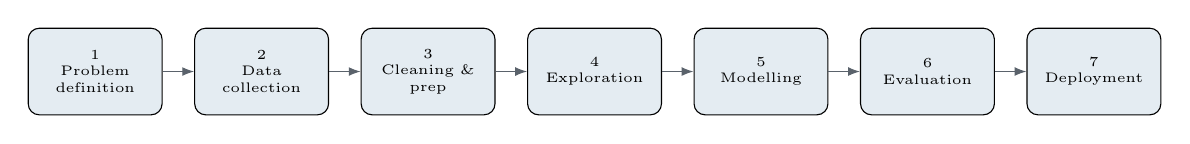
\begin{tikzpicture}[
  node distance=0.4cm,
  s/.style={draw, rounded corners, fill=dsblue!12, minimum width=1.7cm, minimum height=1.1cm, align=center, font=\tiny},
  arr/.style={-{Latex[length=1.5mm]}, dsgray}
]
\node[s] (n1) {1\\Problem\\definition};
\node[s, right=of n1] (n2) {2\\Data\\collection};
\node[s, right=of n2] (n3) {3\\Cleaning \&\\prep};
\node[s, right=of n3] (n4) {4\\Exploration};
\node[s, right=of n4] (n5) {5\\Modelling};
\node[s, right=of n5] (n6) {6\\Evaluation};
\node[s, right=of n6] (n7) {7\\Deployment};
\foreach \a/\b in {n1/n2, n2/n3, n3/n4, n4/n5, n5/n6, n6/n7}
  \draw[arr] (\a) -- (\b);
\end{tikzpicture}
\end{adjustbox}
\end{center}
\vspace{0.3cm}
\trapbox{Stage 3 is most of the work}{Beginners expect modelling to take longest. In practice, collecting and cleaning the data consumes most of a real project --- modelling is often an afternoon.}
\end{frame}

\begin{frame}{Three kinds of data}
The shape of your data decides how much work is needed before you can analyse it.
\begin{table}
\small
\begin{tabularx}{\linewidth}{@{}lXXl@{}}
\toprule
\textbf{Kind} & \textbf{Looks like} & \textbf{Examples} & \textbf{Effort} \\
\midrule
Structured & rows and columns, every row the same shape & CSV, SQL tables & Low \\
Semi-structured & has labels, but rows can differ & JSON, XML, logs & Medium \\
Unstructured & no rows or labels at all & text, images, audio & High \\
\bottomrule
\end{tabularx}
\end{table}
\analogybox{the master chef}{Raw ingredients are raw data. Knives and ovens are programming tools. Recipes are mathematical methods. The plated dish is the decision somebody acts on.}
\end{frame}

\begin{frame}{How the field grew}
\begin{table}
\small
\begin{tabularx}{\linewidth}{@{}lXX@{}}
\toprule
\textbf{Era} & \textbf{Hard part} & \textbf{Typical method} \\
\midrule
Statistics (pre-2000) & collecting data at all & averages, hypothesis tests, by hand \\
Big data (2000--2010) & storing and querying it & databases, Hadoop, SQL \\
Machine learning (2010--now) & choosing what to learn & algorithms find the pattern \\
Generative AI (2020--now) & steering the output & very large models \\
\bottomrule
\end{tabularx}
\end{table}
\vspace{0.3cm}
\keyidea{Early on, a human proposed the pattern and tested it with data. Now the machine proposes the pattern and the human tests it.}
\end{frame}

\begin{frame}{AI, machine learning, deep learning, generative AI}
\begin{center}
\begin{adjustbox}{max width=0.94\linewidth, max height=4.6cm}
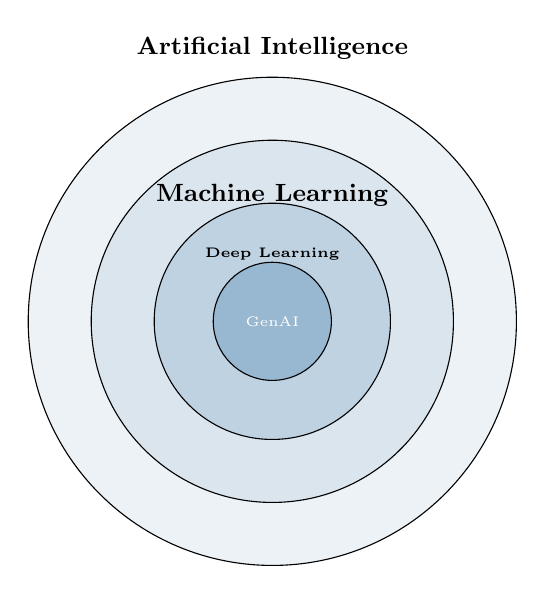
\begin{tikzpicture}
\node[draw, circle, minimum size=6.2cm, fill=dsblue!8] (ai) {};
\node[draw, circle, minimum size=4.6cm, fill=dsblue!16] (ml) {};
\node[draw, circle, minimum size=3.0cm, fill=dsblue!28] (dl) {};
\node[draw, circle, minimum size=1.5cm, fill=dsblue!45, text=white] (gen) {\tiny GenAI};
\node[above=0.1cm of ai.north, anchor=south] {\small\textbf{Artificial Intelligence}};
\node at (0,1.6) {\small\textbf{Machine Learning}};
\node at (0,0.85) {\tiny\textbf{Deep Learning}};
\end{tikzpicture}
\end{adjustbox}
\end{center}
\vspace{-0.2cm}
The useful distinction: \textbf{who writes the rule?} In ordinary programming, you do. In machine learning, the machine works out the rule from examples.
\end{frame}

\begin{frame}{Who does the work}
\begin{table}
\small
\begin{tabularx}{\linewidth}{@{}lXXX@{}}
\toprule
\textbf{Role} & \textbf{Owns} & \textbf{Tools} & \textbf{Delivers} \\
\midrule
Data engineer & getting data in, reliably & SQL, Python, cloud & a trustworthy table \\
Data analyst & explaining what happened & spreadsheets, dashboards & a report \\
Data scientist & predicting what will happen & Python, scikit-learn & a model \\
\bottomrule
\end{tabularx}
\end{table}
\analogybox{the car factory}{The data engineer builds the assembly line. The data analyst counts defects coming off it. The data scientist works out which settings cause fewer defects next month.}
\end{frame}

\begin{frame}{Where you meet it every day}
\begin{columns}[T]
\begin{column}{0.5\textwidth}
\begin{itemize}\small
\item \textbf{Recommendations} --- Netflix, Amazon, Spotify
\item \textbf{Dynamic pricing} --- airlines, ride-hailing
\item \textbf{Fraud detection} --- your bank, every card swipe
\item \textbf{Medical diagnostics} --- radiology
\end{itemize}
\end{column}
\begin{column}{0.5\textwidth}
\begin{itemize}\small
\item \textbf{Demand forecasting} --- retail stock
\item \textbf{Predictive maintenance} --- factories, railways
\item \textbf{Route optimisation} --- maps, delivery
\item \textbf{Credit scoring} --- lenders
\end{itemize}
\end{column}
\end{columns}
\vspace{0.4cm}
\trapbox{A prediction without a range is a guess in a suit}{A number reported without its uncertainty invites a decision it cannot support.}
\end{frame}

\section{Session 2 --- Data Collection \& Pre-Processing}

\begin{frame}{Five ways to collect data}
\begin{table}
\small
\begin{tabularx}{\linewidth}{@{}lXX@{}}
\toprule
\textbf{Route} & \textbf{Use when} & \textbf{Watch out for} \\
\midrule
Internal databases & facts about your own operations & undocumented schemas \\
Files handed to you & someone already extracted it & unknown extraction method \\
APIs & the owner is happy to share & rate limits, format drift \\
Web scraping & no API, but public & terms of service \\
Sensors / surveys & the data does not exist yet & slow and expensive \\
\bottomrule
\end{tabularx}
\end{table}
\end{frame}

\begin{frame}{Sampling: how a sample lies}
\begin{table}
\small
\begin{tabularx}{\linewidth}{@{}lXX@{}}
\toprule
\textbf{Method} & \textbf{How it picks} & \textbf{Risk} \\
\midrule
Random & every row, equal chance & needs the full list \\
Stratified & proportionally from each group & must know the groups \\
Systematic & every $n$th row & fails on repeating patterns \\
Convenience & whatever was easy & \textbf{usually biased, invisibly} \\
\bottomrule
\end{tabularx}
\end{table}
\vspace{0.3cm}
\trapbox{More data does not fix a biased sample}{Doubling a biased sample gives a more confident wrong answer. Only changing \emph{how} you collect fixes bias.}
\end{frame}

\begin{frame}{Why raw data is never usable}
\keyidea{Preprocessing is turning raw data into a table an algorithm can read. It is most of the work in most projects.}
\vspace{0.3cm}
Raw data is messy because it is produced by people and imperfect machines:
\begin{itemize}\small
\item somebody typed their age as 225
\item a sensor dropped offline for four hours
\item one system writes dates one way, another writes them differently
\item a customer pressed \emph{Submit} twice
\item ``Mumbai'', ``mumbai'', ``Bombay'' and ``MUM'' are the same city
\end{itemize}
\end{frame}

\begin{frame}{The order we clean in}
\begin{center}
\begin{adjustbox}{max width=0.94\linewidth, max height=4.6cm}
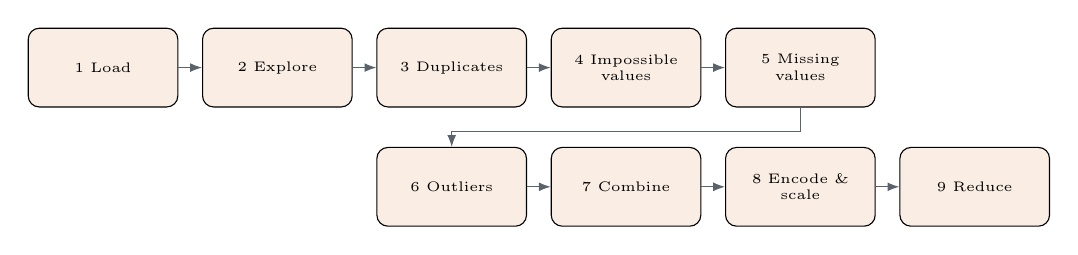
\begin{tikzpicture}[
  s/.style={draw, rounded corners, fill=dsorange!12, minimum width=1.9cm, minimum height=1cm, align=center, font=\tiny},
  arr/.style={-{Latex[length=1.5mm]}, dsgray}
]
\node[s] (a) {1 Load};
\node[s, right=0.3cm of a] (b) {2 Explore};
\node[s, right=0.3cm of b] (c) {3 Duplicates};
\node[s, right=0.3cm of c] (d) {4 Impossible\\values};
\node[s, right=0.3cm of d] (e) {5 Missing\\values};
\node[s, below=0.5cm of c] (f) {6 Outliers};
\node[s, right=0.3cm of f] (g) {7 Combine};
\node[s, right=0.3cm of g] (h) {8 Encode \&\\scale};
\node[s, right=0.3cm of h] (i) {9 Reduce};
\draw[arr] (a)--(b); \draw[arr] (b)--(c); \draw[arr] (c)--(d); \draw[arr] (d)--(e);
\draw[arr] (e.south) -- ++(0,-0.3) -| (f.north);
\draw[arr] (f)--(g); \draw[arr] (g)--(h); \draw[arr] (h)--(i);
\end{tikzpicture}
\end{adjustbox}
\end{center}
\trapbox{Two orderings are not negotiable}{Impossible values before missing values --- an age of 225 must become ``missing'' first. Scaling comes last, only after the data is split for testing.}
\end{frame}

\begin{frame}{Pandas: the spreadsheet that takes orders}
\analogybox{a spreadsheet you talk to}{Instead of dragging to select rows, you say ``give me the rows where city is Mumbai'' --- and it works the same whether there are 20 rows or 20 million.}
\vspace{0.3cm}
Five commands answer almost everything about a new table:
\begin{table}
\small
\begin{tabularx}{\linewidth}{@{}lX@{}}
\toprule
\textbf{Command} & \textbf{Answers} \\
\midrule
\texttt{.shape} & how big is it? \\
\texttt{.head()} & what do the rows look like? \\
\texttt{.info()} & what type is each column, how much is missing? \\
\texttt{.describe()} & what are the numeric columns like? \\
\texttt{.value\_counts()} & what values does a text column hold? \\
\bottomrule
\end{tabularx}
\end{table}
\end{frame}

\begin{frame}{Key takeaways --- Sessions 1--2}
\begin{itemize}
\item Data science is a \textbf{sequence of stages}, not one clever trick.
\item The three ingredients --- programming, mathematics, domain knowledge --- must all be present.
\item Structured, semi-structured and unstructured data cost very different amounts of preparation.
\item A biased sample cannot be fixed by collecting more of it.
\item Cleaning and preparation, not modelling, is where most project time goes.
\end{itemize}
\end{frame}

% ============================================================
\part{Part B --- Making Data Fit to Use}
\frame{\partpage}

\section{Session 3 --- Data Cleaning}

\begin{frame}{Six cleaning jobs, one fixed order}
\begin{center}
\begin{adjustbox}{max width=0.94\linewidth, max height=4.4cm}
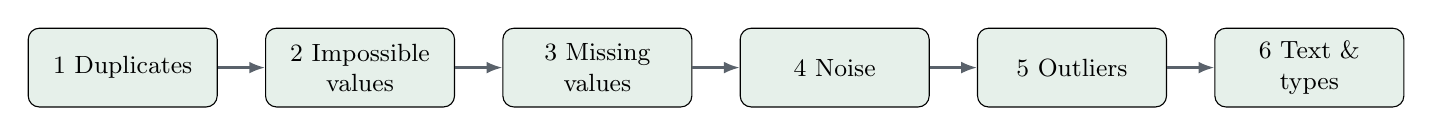
\begin{tikzpicture}[
  s/.style={draw, rounded corners, fill=dsgreen!12, minimum width=2.4cm, minimum height=1cm, align=center, font=\small},
  arr/.style={-{Latex[length=2mm]}, thick, dsgray}
]
\node[s] (a) {1 Duplicates};
\node[s, right=0.6cm of a] (b) {2 Impossible\\values};
\node[s, right=0.6cm of b] (c) {3 Missing\\values};
\node[s, right=0.6cm of c] (d) {4 Noise};
\node[s, right=0.6cm of d] (e) {5 Outliers};
\node[s, right=0.6cm of e] (f) {6 Text \&\\types};
\foreach \x/\y in {a/b, b/c, c/d, d/e, e/f} \draw[arr] (\x) -- (\y);
\end{tikzpicture}
\end{adjustbox}
\end{center}
\trapbox{Impossible is not the same as extreme}{Impossible = it cannot be true (age of 225) --- turn it into missing, then impute it. Extreme = unusual but real (a ₹4,00,000 purchase) --- think hard before touching it.}
\end{frame}

\begin{frame}{Filling missing values}
\analogybox{the missing puzzle piece}{An imputed value is a good guess standing in for a blank. In data science, guessing wrong can ruin a model's accuracy.}
\begin{table}
\small
\begin{tabularx}{\linewidth}{@{}lX@{}}
\toprule
\textbf{Situation} & \textbf{Fill with} \\
\midrule
Numbers, roughly symmetric & mean \\
Numbers, skewed or with extremes & median \\
Text or categories & mode (most common value) \\
Groups that genuinely differ & the group's own median \\
More than \textasciitilde40\% missing & drop the column \\
\bottomrule
\end{tabularx}
\end{table}
\end{frame}

\begin{frame}{Noise, and the smoothing trade-off}
\keyidea{Noise is small random error on top of a real pattern --- not wrong data, just distraction.}
\vspace{0.3cm}
\trapbox{Over-smoothing erases the thing you were looking for}{A wide averaging window removes noise beautifully but also arrives late at every real peak --- and a genuine spike (fraud, a failure) can vanish entirely. The window is a trade between noise and lag; no setting avoids both.}
\end{frame}

\begin{frame}{Detecting outliers: two rules}
\begin{table}
\small
\begin{tabularx}{\linewidth}{@{}lXX@{}}
\toprule
\textbf{Rule} & \textbf{Flags a value if} & \textbf{Use when} \\
\midrule
IQR rule & below $Q_1-1.5\,\mathrm{IQR}$ or above $Q_3+1.5\,\mathrm{IQR}$ & almost always \\
Z-score rule & more than 3 std.\ deviations from the mean & data is roughly bell-shaped \\
\bottomrule
\end{tabularx}
\end{table}
\trapbox{In fraud data, the outliers are the answer}{A pipeline that automatically removes outliers deletes every fraud case you were hired to find --- and reports excellent accuracy on what is left.}
\end{frame}

\section{Session 4 --- Data Integration}

\begin{frame}{Five ways to integrate}
\begin{table}
\footnotesize
\begin{tabularx}{\linewidth}{@{}lXX@{}}
\toprule
\textbf{Approach} & \textbf{Good} & \textbf{Bad} \\
\midrule
Physical (warehouse) & fast queries, one place to look & stale, expensive \\
Virtual (federation) & always current & slow, breaks if a source is down \\
Application-based & no central system & every app must know every other \\
Middleware & apps stay simple & middleware is a single point of failure \\
Manual & works today & slow, unrepeatable, error-prone \\
\bottomrule
\end{tabularx}
\end{table}
\analogybox{the wedding guest list}{Two partners keep guests in different formats. Integration is the painful merge into one list --- and deciding whether ``R. Sharma'' and ``Raj Sharma'' are the same person is the whole difficulty.}
\end{frame}

\begin{frame}{Stacking vs linking}
\begin{table}
\small
\begin{tabularx}{\linewidth}{@{}lXl@{}}
\toprule
\textbf{Operation} & \textbf{Question it answers} & \textbf{Function} \\
\midrule
Stacking & ``here are more rows of the same thing'' & \texttt{concat} \\
Linking & ``here is extra info about the same things'' & \texttt{merge} \\
\bottomrule
\end{tabularx}
\end{table}
\vspace{0.3cm}
\keyidea{Two months of sales: stack. Customers and their orders: link.}
\end{frame}

\begin{frame}{The four join types}
\begin{table}
\small
\begin{tabularx}{\linewidth}{@{}lXX@{}}
\toprule
\textbf{Type} & \textbf{Keeps} & \textbf{Use when} \\
\midrule
inner & only rows matching in both & you need complete records \\
left & all left rows, blanks where unmatched & the left table is your population \\
right & all right rows & rare, usually a relabelled left \\
outer & everything from both & looking for what does not match \\
\bottomrule
\end{tabularx}
\end{table}
\trapbox{A join that changes the row count is a claim}{Shrinking says some records had no match. Growing says a key is not unique. Always check the row count before and after.}
\end{frame}

\section{Session 5 --- Data Transformation}

\begin{frame}{Why scale matters}
\keyidea{Many algorithms measure distance between rows. A column with big numbers dominates that distance, whatever it means.}
\analogybox{judging a contest in different units}{One judge scores out of 10, another out of 1{,}000. Add the scores and the second judge decides the winner every time --- not because their opinion is better, but because their scale is bigger.}
\end{frame}

\begin{frame}{Five transformers}
\begin{table}
\footnotesize
\begin{tabularx}{\linewidth}{@{}lXl@{}}
\toprule
\textbf{Tool} & \textbf{Produces} & \textbf{Works on} \\
\midrule
MinMaxScaler & values between 0 and 1 & columns \\
StandardScaler & mean 0, std.\ dev.\ 1 & columns \\
RobustScaler & centred on median, scaled by IQR & columns \\
Normalizer & each row rescaled to length 1 & \textbf{rows} \\
Binarizer & 0 or 1, split at a threshold & columns \\
\bottomrule
\end{tabularx}
\end{table}
\trapbox{Which algorithms actually need scaling}{Distance-based (kNN, K-Means, SVM) and neural nets: yes. Tree-based models (decision trees, random forests): no --- a tree asks ``is age $>$ 30?'', and units don't change that split.}
\end{frame}

\begin{frame}{Encoding categories}
\begin{table}
\small
\begin{tabularx}{\linewidth}{@{}lXl@{}}
\toprule
\textbf{Kind} & \textbf{Meaning} & \textbf{Encode with} \\
\midrule
Nominal & no order (city, colour) & one-hot \\
Ordinal & a real order (small $<$ medium $<$ large) & ordinal encoding \\
The target & what you predict & label encoding \\
\bottomrule
\end{tabularx}
\end{table}
\trapbox{Never label-encode a nominal feature}{Label-encode city as Delhi=0, Mumbai=1, Pune=2 and the algorithm believes Pune is ``twice'' Mumbai. None of that is true.}
\end{frame}

\begin{frame}{The train--test split, and leakage}
\analogybox{practice papers and the real exam}{The training set is practice papers with answers. The test set is the exam. A model tested on its own training data is a student marking their own homework.}
\vspace{0.2cm}
\trapbox{The test set is spent after one use}{Every peek at the test score while choosing a model leaks a little information into your choices. Split off the test set, do all tuning by cross-validation on the training data, and look at the test set once.}
\end{frame}

\section{Session 6 --- Data Reduction \& Discretization}

\begin{frame}{Three kinds of reduction}
\begin{center}
\begin{adjustbox}{max width=0.9\linewidth, max height=4.2cm}
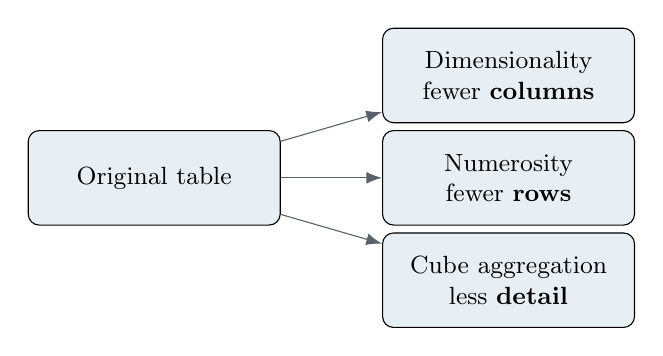
\begin{tikzpicture}[
  s/.style={draw, rounded corners, fill=dsblue!10, minimum width=3.2cm, minimum height=1.2cm, align=center, font=\small},
]
\node[s] (d) at (0,0) {Original table};
\node[s] (a) at (4.5,1.3) {Dimensionality\\fewer \textbf{columns}};
\node[s] (b) at (4.5,0) {Numerosity\\fewer \textbf{rows}};
\node[s] (c) at (4.5,-1.3) {Cube aggregation\\less \textbf{detail}};
\draw[-{Latex[length=2mm]}, dsgray] (d) -- (a);
\draw[-{Latex[length=2mm]}, dsgray] (d) -- (b);
\draw[-{Latex[length=2mm]}, dsgray] (d) -- (c);
\end{tikzpicture}
\end{adjustbox}
\end{center}
\end{frame}

\begin{frame}{Feature selection: three families}
\begin{table}
\small
\begin{tabularx}{\linewidth}{@{}lXl@{}}
\toprule
\textbf{Family} & \textbf{How it decides} & \textbf{Example} \\
\midrule
Filter & score each column vs.\ target, alone & correlation, chi-square \\
Wrapper & retrain repeatedly, add/remove columns & recursive feature elimination \\
Embedded & the model selects while training & Lasso, tree importance \\
\bottomrule
\end{tabularx}
\end{table}
\end{frame}

\begin{frame}{PCA: compressing columns}
\analogybox{the shadow}{Hold a teapot to a lamp; the shadow is 2-D, yet you can still tell it is a teapot, because you chose the angle that keeps the most information. Where it breaks down: you cannot tell which side the handle is on.}
\trapbox{PCA costs you the ability to explain the model}{After PCA, inputs are ``component 1'', ``component 2''. If asked ``why was this loan refused?'', that answer means nothing to the applicant.}
\end{frame}

\begin{frame}{Discretization: top-down vs bottom-up}
\begin{table}
\small
\begin{tabularx}{\linewidth}{@{}lXl@{}}
\toprule
\textbf{Family} & \textbf{Starts from} & \textbf{Example} \\
\midrule
Top-down (splitting) & the whole range, one bin & equal-width, equal-frequency \\
Bottom-up (merging) & every value its own bin & chi-merge \\
\bottomrule
\end{tabularx}
\end{table}
\keyidea{Bin when the categories mean something to a human. Do not bin just to tidy up --- binning always destroys information.}
\end{frame}

\begin{frame}{Key takeaways --- Sessions 3--6}
\begin{itemize}
\item Clean in a fixed order: duplicates, impossible values, missing values, noise, outliers, text/types.
\item Check the row count after every join --- silently doubled or shrunk data is the costliest undetected error.
\item Split before you scale; never label-encode a nominal feature.
\item Reduction always throws something away --- know what, and be able to justify it.
\end{itemize}
\end{frame}

% ============================================================
\part{Part C --- Understanding Data}
\frame{\partpage}

\section{Session 7 --- Descriptive Statistics}

\begin{frame}{Mean, median, mode}
\begin{table}
\small
\begin{tabularx}{\linewidth}{@{}lXX@{}}
\toprule
\textbf{Measure} & \textbf{What it is} & \textbf{Answers} \\
\midrule
Mean & add everything, divide by count & if shared equally, how much each? \\
Median & sort, take the middle value & what does the middle person have? \\
Mode & most frequent value & what is most common? \\
\bottomrule
\end{tabularx}
\end{table}
\analogybox{the pub and the billionaire}{Ten people in a pub average ₹5 lakh in wealth. A billionaire walks in --- the average leaps past ₹90 crore, while the median barely moves. Which number describes ``how rich are the people in this pub''?}
\end{frame}

\begin{frame}{Spread: four measures}
\begin{table}
\small
\begin{tabularx}{\linewidth}{@{}lXl@{}}
\toprule
\textbf{Measure} & \textbf{Computed as} & \textbf{Sensitive to outliers?} \\
\midrule
Range & max $-$ min & extremely \\
Variance & average squared distance from mean & yes \\
Std.\ deviation & $\sqrt{\text{variance}}$ & yes \\
IQR & $Q_3-Q_1$, the middle half & no \\
\bottomrule
\end{tabularx}
\end{table}
\analogybox{two archers}{Both archers average dead centre. One puts every arrow within a coin's width of the bullseye; the other scatters corner to corner. Identical averages, only one can actually hit a target.}
\end{frame}

\begin{frame}{Skewness and kurtosis}
\begin{table}
\small
\begin{tabularx}{\linewidth}{@{}lXX@{}}
\toprule
\textbf{Skewness} & \textbf{Shape} & \textbf{Mean vs median} \\
\midrule
$\approx 0$ & symmetric & equal \\
positive & long tail right & mean $>$ median \\
negative & long tail left & mean $<$ median \\
\bottomrule
\end{tabularx}
\end{table}
\vspace{0.2cm}
\keyidea{A quick check needing no calculation: compare the mean and the median. If the mean is noticeably higher, the data is right-skewed.}
\end{frame}

\begin{frame}{Z-scores: comparing across scales}
\[ z = \frac{\text{value} - \text{mean}}{\text{standard deviation}} \]
\keyidea{A z-score says how many standard deviations a value sits from the mean --- so you can compare things measured on completely different scales.}
\trapbox{Most real data is not normally distributed}{Financial, biological and web-traffic data routinely break the bell-curve assumption. Check before you assume: plot a histogram, compare mean and median, look at kurtosis.}
\end{frame}

\section{Session 8 --- EDA \& Visualization}

\begin{frame}{The first pass: five questions in order}
\begin{table}
\small
\begin{tabularx}{\linewidth}{@{}cXl@{}}
\toprule
\# & \textbf{Question} & \textbf{Tool} \\
\midrule
1 & How big is it, what type is each column? & \texttt{.shape}, \texttt{.info()} \\
2 & What does each column look like alone? & histogram, box plot \\
3 & What is missing or impossible? & \texttt{.isna().sum()} \\
4 & Which columns move together? & scatter, correlation \\
5 & What differs between groups? & \texttt{groupby}, pivot \\
\bottomrule
\end{tabularx}
\end{table}
\analogybox{the doctor's examination}{A doctor does not begin with surgery. Most checks find nothing --- that is the point --- and occasionally one finds something that changes the whole plan.}
\end{frame}

\begin{frame}{Choosing the chart}
\begin{table}
\footnotesize
\begin{tabularx}{\linewidth}{@{}Xl@{}}
\toprule
\textbf{Question} & \textbf{Chart} \\
\midrule
How is one number spread out? & histogram \\
Centre, spread, outliers? & box plot \\
How many of each category? & bar chart \\
Do two numbers move together? & scatter plot \\
Does a number differ by group? & box plot by group \\
How do many numeric columns relate? & heatmap \\
\bottomrule
\end{tabularx}
\end{table}
\trapbox{Correlation only measures straight-line relationships}{A curved but perfect relationship can score a Pearson correlation near zero. Look at the scatter plot, not just the number.}
\end{frame}

\begin{frame}{Correlation is not causation}
\keyidea{A correlation is a question worth investigating, never an answer.}
\vspace{0.3cm}
Three things a correlation can mean:
\begin{enumerate}
\item A causes B
\item B causes A
\item \textbf{C causes both --- usually this one (a confounder)}
\end{enumerate}
\vspace{0.2cm}
\analogybox{ice cream and drowning}{Ice cream sales correlate strongly with drowning deaths. Ice cream does not cause drowning --- hot weather causes both.}
\end{frame}

\begin{frame}{Pivot tables, and checking the count behind an average}
\trapbox{Always check the counts behind an average}{An average computed from two rows sits in a pivot table looking exactly as authoritative as one computed from two hundred. Print the count table alongside any pivot of means.}
\end{frame}

\begin{frame}{Key takeaways --- Sessions 7--8}
\begin{itemize}
\item Never report a centre without a spread --- and look at the shape too.
\item Compare mean vs median as a free, instant skew check.
\item Every chart should answer a question you asked \emph{before} drawing it.
\item Correlation is a lead to investigate, not a finding to report.
\end{itemize}
\end{frame}

% ============================================================
\part{Part D --- Learning From Data}
\frame{\partpage}

\section{Session 9 --- Supervised Learning}

\begin{frame}{Supervised learning}
\keyidea{Supervised learning trains an algorithm on historical data where the answer is already known.}
\analogybox{flashcards}{The front of the card is the input (features). The back is the answer (label). Learning is guessing, flipping the card, and adjusting --- until you get it right every time.}
\end{frame}

\begin{frame}{Regression or classification?}
\begin{table}
\small
\begin{tabularx}{\linewidth}{@{}lXX@{}}
\toprule
& \textbf{Target is} & \textbf{Examples} \\
\midrule
Regression & a number & house price, tomorrow's temperature \\
Classification & a category & spam or not, which disease \\
\bottomrule
\end{tabularx}
\end{table}
\end{frame}

\begin{frame}{Reading a coefficient correctly}
\keyidea{A coefficient is the effect of that feature while every other feature is held constant.}
\vspace{0.3cm}
``Each extra bedroom adds ₹4 lakh'' is wrong. \textbf{``Each extra bedroom adds ₹4 lakh, comparing houses of the same area and age''} is right --- and a completely different claim.
\end{frame}

\begin{frame}{Three regression metrics}
\begin{table}
\small
\begin{tabularx}{\linewidth}{@{}lXl@{}}
\toprule
\textbf{Metric} & \textbf{What it is} & \textbf{Character} \\
\midrule
MAE & average size of the error & treats all errors evenly \\
RMSE & square root of avg.\ squared error & punishes large errors harder \\
R\textsuperscript{2} & share of variation explained & 1.0 perfect, 0 = no better than the mean \\
\bottomrule
\end{tabularx}
\end{table}
\trapbox{Always compare against a baseline}{R\textsuperscript{2} of 0 means "no better than always guessing the average." Run the baseline before trusting any score.}
\end{frame}

\section{Session 10 --- Unsupervised Learning \& Clustering}

\begin{frame}{Clustering has no answer key}
\begin{table}
\small
\begin{tabularx}{\linewidth}{@{}lXX@{}}
\toprule
& \textbf{Supervised} & \textbf{Unsupervised} \\
\midrule
Data & $X$ and $y$ & $X$ only \\
Can you measure accuracy? & yes & \textbf{no} \\
Fails by & predicting badly & producing groups that mean nothing \\
\bottomrule
\end{tabularx}
\end{table}
\analogybox{sorting the laundry}{Nobody told you the categories. Somebody else would make different piles --- by fabric instead of colour. Neither is wrong. Several defensible answers, no marking scheme.}
\end{frame}

\begin{frame}{K-Means, in three steps}
\begin{center}
\begin{adjustbox}{max width=0.85\linewidth, max height=4.2cm}
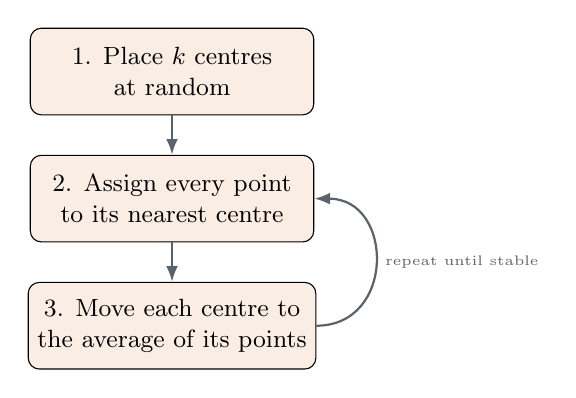
\begin{tikzpicture}[
  s/.style={draw, rounded corners, fill=dsorange!12, minimum width=3.6cm, minimum height=1.1cm, align=center, font=\small},
  arr/.style={-{Latex[length=2mm]}, thick, dsgray}
]
\node[s] (a) {1. Place $k$ centres\\at random};
\node[s, below=0.5cm of a] (b) {2. Assign every point\\to its nearest centre};
\node[s, below=0.5cm of b] (c) {3. Move each centre to\\the average of its points};
\draw[arr] (a) -- (b);
\draw[arr] (b) -- (c);
\draw[arr] (c.east) to[out=0,in=0,looseness=1.6] node[right,font=\tiny]{repeat until stable} (b.east);
\end{tikzpicture}
\end{adjustbox}
\end{center}
\trapbox{Scale first, always}{K-Means measures straight-line distance. An unscaled column with big numbers decides every cluster on its own.}
\end{frame}

\begin{frame}{Choosing $k$}
\begin{table}
\small
\begin{tabularx}{\linewidth}{@{}lX@{}}
\toprule
\textbf{Method} & \textbf{Idea} \\
\midrule
Elbow method & inertia always falls with more clusters --- look for the bend where it stops paying \\
Silhouette score & how much closer a point is to its own cluster than the next nearest --- higher is genuinely better \\
\bottomrule
\end{tabularx}
\end{table}
\trapbox{Clustering always returns clusters}{Ask K-Means for 4 groups in pure random noise and it will confidently return 4 groups. A tidy chart is not evidence that groups exist.}
\end{frame}

\section{Session 11 --- Model Evaluation}

\begin{frame}{Overfitting and underfitting}
\begin{table}
\small
\begin{tabularx}{\linewidth}{@{}lXX@{}}
\toprule
& \textbf{Underfitting} & \textbf{Overfitting} \\
\midrule
Model is & too simple & too complex \\
Training score & poor & excellent \\
Test score & poor & \textbf{poor} \\
It has & missed the pattern & memorised the noise \\
\bottomrule
\end{tabularx}
\end{table}
\analogybox{three students revising}{One skimmed a page (bad at practice and the exam). One memorised the practice papers word for word (perfect at practice, lost on the real exam). Only the good student, who learned the method, does well at both.}
\end{frame}

\begin{frame}{Why one split is not enough}
\keyidea{A single train-test split gives you one number, and that number depends on which rows happened to land in the test set.}
\trapbox{Report a range, not a point}{If single splits vary by 0.15 in score, and your model beats a colleague's by 0.03, you have shown nothing. Cross-validate and report the spread.}
\end{frame}

\begin{frame}{K-fold cross-validation}
\begin{center}
\begin{adjustbox}{max width=0.92\linewidth, max height=4cm}
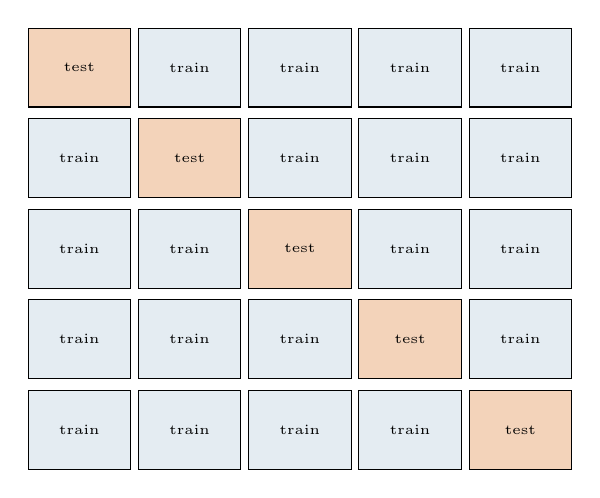
\begin{tikzpicture}[
  f/.style={draw, minimum width=1.3cm, minimum height=1cm, font=\tiny, align=center},
  test/.style={f, fill=dsorange!30},
  train/.style={f, fill=dsblue!12}
]
\foreach \row/\testcol in {0/1,1/2,2/3,3/4,4/5}{
  \foreach \col in {1,...,5}{
    \ifnum\col=\testcol
      \node[test] at (\col*1.4, -\row*1.15) {test};
    \else
      \node[train] at (\col*1.4, -\row*1.15) {train};
    \fi
  }
}
\end{tikzpicture}
\end{adjustbox}
\end{center}
\keyidea{Every row is tested exactly once. Report the average score AND its spread across folds.}
\end{frame}

\begin{frame}{The test set is spent after one use}
\trapbox{Tuning on the test set invalidates the score}{Every time you look at the test score and change something because of it, you leak information into your choices. The discipline: split off the test set, tune only with cross-validation on training data, look at the test set once, at the very end.}
\end{frame}

\section{Session 12 --- Model Saving \& Deployment}

\begin{frame}{Save the pipeline, not the model}
\keyidea{A model saved without its scaler and encoder will accept raw input and return confident, wrong predictions --- and nothing will raise an error.}
\analogybox{the recipe and the cooking}{Training is developing the recipe (weeks of work). Saving is writing it down. Prediction is cooking (twenty minutes). You do not redevelop the recipe every time someone orders dinner.}
\end{frame}

\begin{frame}{Offline vs online deployment}
\begin{table}
\footnotesize
\begin{tabularx}{\linewidth}{@{}lXX@{}}
\toprule
& \textbf{Offline (batch)} & \textbf{Online (live)} \\
\midrule
When it runs & on a schedule & the moment someone asks \\
Input/output & a whole file & one row / one answer \\
Needs a server always on? & no & yes \\
Good for & churn scores, restock lists & loan decisions, fraud checks \\
\bottomrule
\end{tabularx}
\end{table}
\keyidea{Most projects should start offline. If a nightly file of predictions solves the problem, you have avoided servers, uptime and latency entirely.}
\end{frame}

\begin{frame}{What breaks after launch}
\begin{table}
\footnotesize
\begin{tabularx}{\linewidth}{@{}lX@{}}
\toprule
\textbf{Problem} & \textbf{What happens} \\
\midrule
Data drift & inputs shift over time \\
Concept drift & the relationship itself shifts \\
Schema change & an upstream column is renamed \\
Version drift & the library is upgraded under the model \\
Extrapolation & users enter values outside the training range \\
\bottomrule
\end{tabularx}
\end{table}
\trapbox{Validate at the door}{A model will happily predict a price for a house of $-50$ square feet. The input layer, not the model, is where you catch nonsense.}
\end{frame}

\begin{frame}{Key takeaways --- Sessions 9--12}
\begin{itemize}
\item A coefficient's meaning always includes ``holding everything else constant.''
\item Clustering has no ground truth --- justify the result, don't just trust the score.
\item Cross-validate and report the spread; one split is one opinion.
\item Save the whole pipeline; validate inputs; expect the world to drift after launch.
\end{itemize}
\end{frame}

% ============================================================
\part{Part E --- Data at Scale}
\frame{\partpage}

\section{Session 13 --- Big Data Fundamentals}

\begin{frame}{The five Vs}
\begin{table}
\footnotesize
\begin{tabularx}{\linewidth}{@{}lX@{}}
\toprule
\textbf{V} & \textbf{The problem it creates} \\
\midrule
Volume & does not fit in memory or on one disk \\
Velocity & cannot store it before the next batch arrives \\
Variety & many shapes need different handling \\
Veracity & how much can you trust it \\
Value & most of it is never used \\
\bottomrule
\end{tabularx}
\end{table}
\keyidea{Only one of these is usually your actual problem. A library with a volume problem needs a bigger building; one with a velocity problem needs a faster door.}
\end{frame}

\begin{frame}{Where one machine stops being enough}
\keyidea{``Big data'' is not a size, it is a symptom --- the point where one machine stops being enough. That point arrives far later than most people think.}
\trapbox{Try these before you build a cluster}{Chunking, selecting only needed columns, and fixing dtypes routinely turn a ``we need Spark'' problem back into a laptop problem. Spend a day on these first.}
\end{frame}

\begin{frame}{Four types of analytics}
\begin{center}
\begin{adjustbox}{max width=0.92\linewidth, max height=2.2cm}
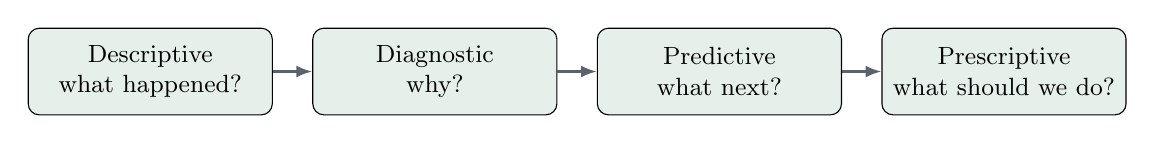
\begin{tikzpicture}[
  s/.style={draw, rounded corners, fill=dsgreen!12, minimum width=3.1cm, minimum height=1.1cm, align=center, font=\small},
  arr/.style={-{Latex[length=2mm]}, thick, dsgray}
]
\node[s] (a) {Descriptive\\what happened?};
\node[s, right=0.5cm of a] (b) {Diagnostic\\why?};
\node[s, right=0.5cm of b] (c) {Predictive\\what next?};
\node[s, right=0.5cm of c] (d) {Prescriptive\\what should we do?};
\foreach \x/\y in {a/b,b/c,c/d} \draw[arr] (\x)--(\y);
\end{tikzpicture}
\end{adjustbox}
\end{center}
\vspace{0.3cm}
Increasing order of difficulty and value --- descriptive is a \texttt{groupby}; prescriptive needs a prediction \emph{and} a judgement call.
\end{frame}

\begin{frame}{How HDFS works}
\begin{table}
\small
\begin{tabularx}{\linewidth}{@{}lX@{}}
\toprule
\textbf{Idea} & \textbf{What it means} \\
\midrule
Blocks & the file is cut into fixed-size pieces (\textasciitilde128 MB) \\
Replication & every block stored on \textbf{three} different machines \\
Write once & files are appended to, never edited in the middle \\
\bottomrule
\end{tabularx}
\end{table}
\trapbox{HDFS is terrible at small files}{A million tiny files use a million entries in the NameNode's in-memory index --- exhausting it long before the disks fill up. Combine small files into large ones before storing.}
\end{frame}

\section{Session 14 --- Distributed Data Processing}

\begin{frame}{MapReduce: three steps}
\begin{table}
\small
\begin{tabularx}{\linewidth}{@{}lXXl@{}}
\toprule
\textbf{Step} & \textbf{Input} & \textbf{Output} & \textbf{Runs} \\
\midrule
Map & one chunk & many (key, value) pairs & in parallel \\
Shuffle & all pairs & grouped by key & across the network \\
Reduce & values for one key & one result per key & in parallel \\
\bottomrule
\end{tabularx}
\end{table}
\analogybox{counting votes}{A hundred counters each tally their own box (map). Tallies for each party are gathered together (shuffle). One person adds up each party's tallies (reduce) --- tiny, because it works on tallies, not ballots.}
\end{frame}

\begin{frame}{The combiner: why the shuffle is expensive}
\keyidea{Map and reduce run locally. The shuffle moves data between machines --- hundreds of times slower than memory.}
\trapbox{Not every reducer can be combined}{\texttt{sum}, \texttt{min}, \texttt{max} and \texttt{count} are safe to pre-aggregate locally. \texttt{average} is not --- the average of averages of unequal groups is wrong. Fix: carry (sum, count) through the shuffle.}
\end{frame}

\begin{frame}{Why Spark replaced Hadoop MapReduce}
\begin{table}
\small
\begin{tabularx}{\linewidth}{@{}lXX@{}}
\toprule
& \textbf{Hadoop MapReduce} & \textbf{Apache Spark} \\
\midrule
Between stages & writes to disk & keeps data in memory \\
Multi-pass work & very slow & fast \\
Interactive queries & no & yes \\
\bottomrule
\end{tabularx}
\end{table}
\keyidea{One pass: barely any difference. Thirty passes --- what training a model looks like --- Spark wins outright.}
\end{frame}

\begin{frame}{Lazy evaluation}
\begin{table}
\small
\begin{tabularx}{\linewidth}{@{}lXl@{}}
\toprule
\textbf{Kind} & \textbf{Examples} & \textbf{Runs immediately?} \\
\midrule
Transformation & filter, select, groupBy, join & no --- recorded \\
Action & show, count, collect, write & \textbf{yes} --- executes the plan \\
\bottomrule
\end{tabularx}
\end{table}
\trapbox{Lazy evaluation moves your errors}{A typo in a column name may not surface until an action runs, possibly many lines later. When timing Spark code, time the action.}
\end{frame}

\begin{frame}{When not to use Spark}
\trapbox{Use Spark when the data does not fit, not when it feels large}{Spark pays a real cost before doing any work at all --- roughly 7 seconds of pure startup and shuffle overhead. It does not earn that back on a 200 MB CSV, however important that CSV is.}
\end{frame}

\section{Session 15 --- NoSQL \& Visualization at Scale}

\begin{frame}{Why NoSQL exists}
\begin{table}
\small
\begin{tabularx}{\linewidth}{@{}lXX@{}}
\toprule
& \textbf{Relational (SQL)} & \textbf{NoSQL} \\
\midrule
Shape decided & before you store anything & as you store \\
Scales by & a bigger machine & more machines \\
Best for & money, bookings & logs, profiles, catalogues \\
\bottomrule
\end{tabularx}
\end{table}
\analogybox{the filing cabinet and the folders}{A filing cabinet holds identical labelled forms --- tidy, but a document that does not fit needs the whole form redesigned. A folder system holds whatever each case needs --- nothing rejected, but you can no longer assume any two folders match.}
\end{frame}

\begin{frame}{The four NoSQL families}
\begin{table}
\small
\begin{tabularx}{\linewidth}{@{}lXl@{}}
\toprule
\textbf{Family} & \textbf{Best at} & \textbf{Example} \\
\midrule
Document & flexible, nested records & MongoDB \\
Wide-column & huge volume, known queries & Cassandra \\
Key--value & caching, sessions & Redis \\
Graph & networks, recommendations & Neo4j \\
\bottomrule
\end{tabularx}
\end{table}
\end{frame}

\begin{frame}{The CAP theorem}
\keyidea{When a distributed database's machines cannot talk to each other, you must choose between a possibly stale answer and no answer.}
\trapbox{This is a business decision, not a technical one}{For a bank balance: refuse to answer rather than risk staleness --- choose consistency. For a page view counter: a thirty-second-old count beats a blank page --- choose availability.}
\end{frame}

\begin{frame}{Charts at scale}
\keyidea{Draw ten million dots and you get a solid rectangle. Aggregate or bin before you plot --- never send raw rows to the chart.}
\trapbox{A sample must be random}{\texttt{df.head(10000)} is not a sample --- it is whatever was written first, usually ordered by time or ID. Use a genuine random sample, and label the margin of error.}
\end{frame}

\section{Session 16 --- Capstone Project}

\begin{frame}{Fix the success criterion before modelling}
\keyidea{A finished project is a question, an honest answer, and a statement of what the answer cannot support.}
\trapbox{Choosing the metric after seeing results is not evaluation, it is rationalisation}{Write the target down before touching the data: e.g. ``catch 60\% of churners while contacting under 30\% of customers.'' Then judge the model against that number, not against 1.0.}
\end{frame}

\begin{frame}{Association rules: support, confidence, lift}
\begin{table}
\small
\begin{tabularx}{\linewidth}{@{}lXl@{}}
\toprule
\textbf{Measure} & \textbf{Question} & \textbf{Formula} \\
\midrule
Support & how often does this happen at all? & count(both) / total \\
Confidence & when left happens, how often right? & support(both) / support(left) \\
Lift & more likely than chance? & confidence / support(right) \\
\bottomrule
\end{tabularx}
\end{table}
\trapbox{Confidence alone will fool you}{A rule pointing at a very common item gets high confidence automatically. Lift near or below 1 means the rule found nothing.}
\end{frame}

\begin{frame}{Test the claim, don't just draw it}
\keyidea{A box plot showing two groups apart is a hypothesis, not a finding. A p-value puts a number on how likely the gap is chance.}
\trapbox{A p-value is not the size of an effect}{With enough rows, even a trivial difference produces a tiny p-value. Always report the effect size next to it --- ``churners make 1.4 more calls on average (p $<$ 0.001)'' is a finding; ``p $<$ 0.001'' alone is not.}
\end{frame}

\begin{frame}{Responsible delivery}
\begin{table}
\footnotesize
\begin{tabularx}{\linewidth}{@{}lX@{}}
\toprule
\textbf{Question} & \textbf{Before shipping} \\
\midrule
Who could be harmed by a wrong prediction? & name the expensive error \\
Does it treat groups differently? & check error rate per group, not just overall \\
Could you explain a decision to the person it affected? & if the answer is ``component 1 was low,'' reconsider \\
\bottomrule
\end{tabularx}
\end{table}
\end{frame}

\begin{frame}{Key takeaways --- Sessions 13--16}
\begin{itemize}
\item Big data is a symptom, not a size --- measure before reaching for a cluster.
\item MapReduce is map, shuffle, reduce; the shuffle is the expensive part.
\item NoSQL trades a fixed schema for flexibility --- and CAP is a business choice.
\item A finished project states plainly what its result cannot support.
\end{itemize}
\end{frame}

\section*{Closing}

\begin{frame}{Sixteen sessions, one sentence each}
\begin{columns}[T]
\begin{column}{0.5\textwidth}
\begin{enumerate}\footnotesize
\item Data science turns facts into decisions
\item Load and look before you touch
\item Clean in a fixed order
\item Join carefully; check row counts
\item Split before you scale; never leak
\item Fewer columns is often better
\item Report centre, spread \emph{and} shape
\item Every chart answers a question
\end{enumerate}
\end{column}
\begin{column}{0.5\textwidth}
\begin{enumerate}\footnotesize
\setcounter{enumi}{8}
\item Beat a baseline, always
\item Clustering has no answer key
\item One split is one opinion
\item Save the pipeline; watch for drift
\item Big data is a symptom, not a size
\item Map, shuffle, reduce
\item NoSQL trades schema for flexibility
\item State what your result cannot support
\end{enumerate}
\end{column}
\end{columns}
\end{frame}

\begin{frame}[standout]
Thank you.
\end{frame}

\end{document}
